\clearpage
\subsection{Hidden-State Depth}
\begin{figure}[H]\centering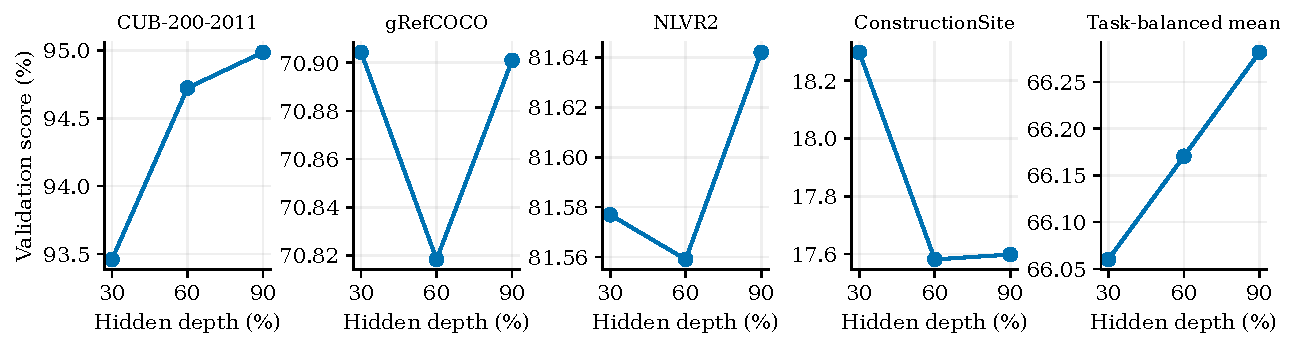
\includegraphics[width=\textwidth]{figures/hidden_depth.pdf}
\caption{Validation low-budget scores at 30\%, 60\% and 90\% relative hidden depth. Each task averages its 4 model pairs, and the final panel averages the 4 tasks equally. All three settings use the 4M student, width 512, learning rate 0.001, 4-state targets and natural sampling. Thus, only hidden depth changes. These are the first stage of the sequential search, not additional sweeps around the final 8M setting.}\end{figure}
Relative depth makes models with different layer counts comparable: the chosen position is rounded upward within the model's recorded sequence of hidden states. Larger depth need not improve every task, so the shared depth is chosen by the task-balanced validation mean. The curve is shown without smoothing or uncertainty bands because each setting uses seed 42.
\subsection{What the Five Input Ablations Establish}
The five input types are image features (I), task text (T), specialist hidden state (H), confidence (C) and prediction summary (P). Table~\ref{tab:ablation} contains earlier one-input removals: I/T/H/C on GroundingDINO and C/P on ResNet and BEiT3. These comparisons cover all five input types across their applicable model pairs, but do not form a five-way removal study of the final shared router. Image-only tasks have no task-text branch. Removing an input also changes the head's input dimension.

The main shared-setting study deliberately retains image and hidden features and includes text whenever the task has it. Consequently, the existing results do not establish that each of its five inputs is individually necessary. The code supplies separate final-setting removal configurations for future runs; unrun settings have no reported scores. Table~\ref{tab:ablation} should be interpreted only against the reference within each block.
